\newpage
\subsection{Login Page}\hfill

%For the main pages put a mockup and describe it in detail.

%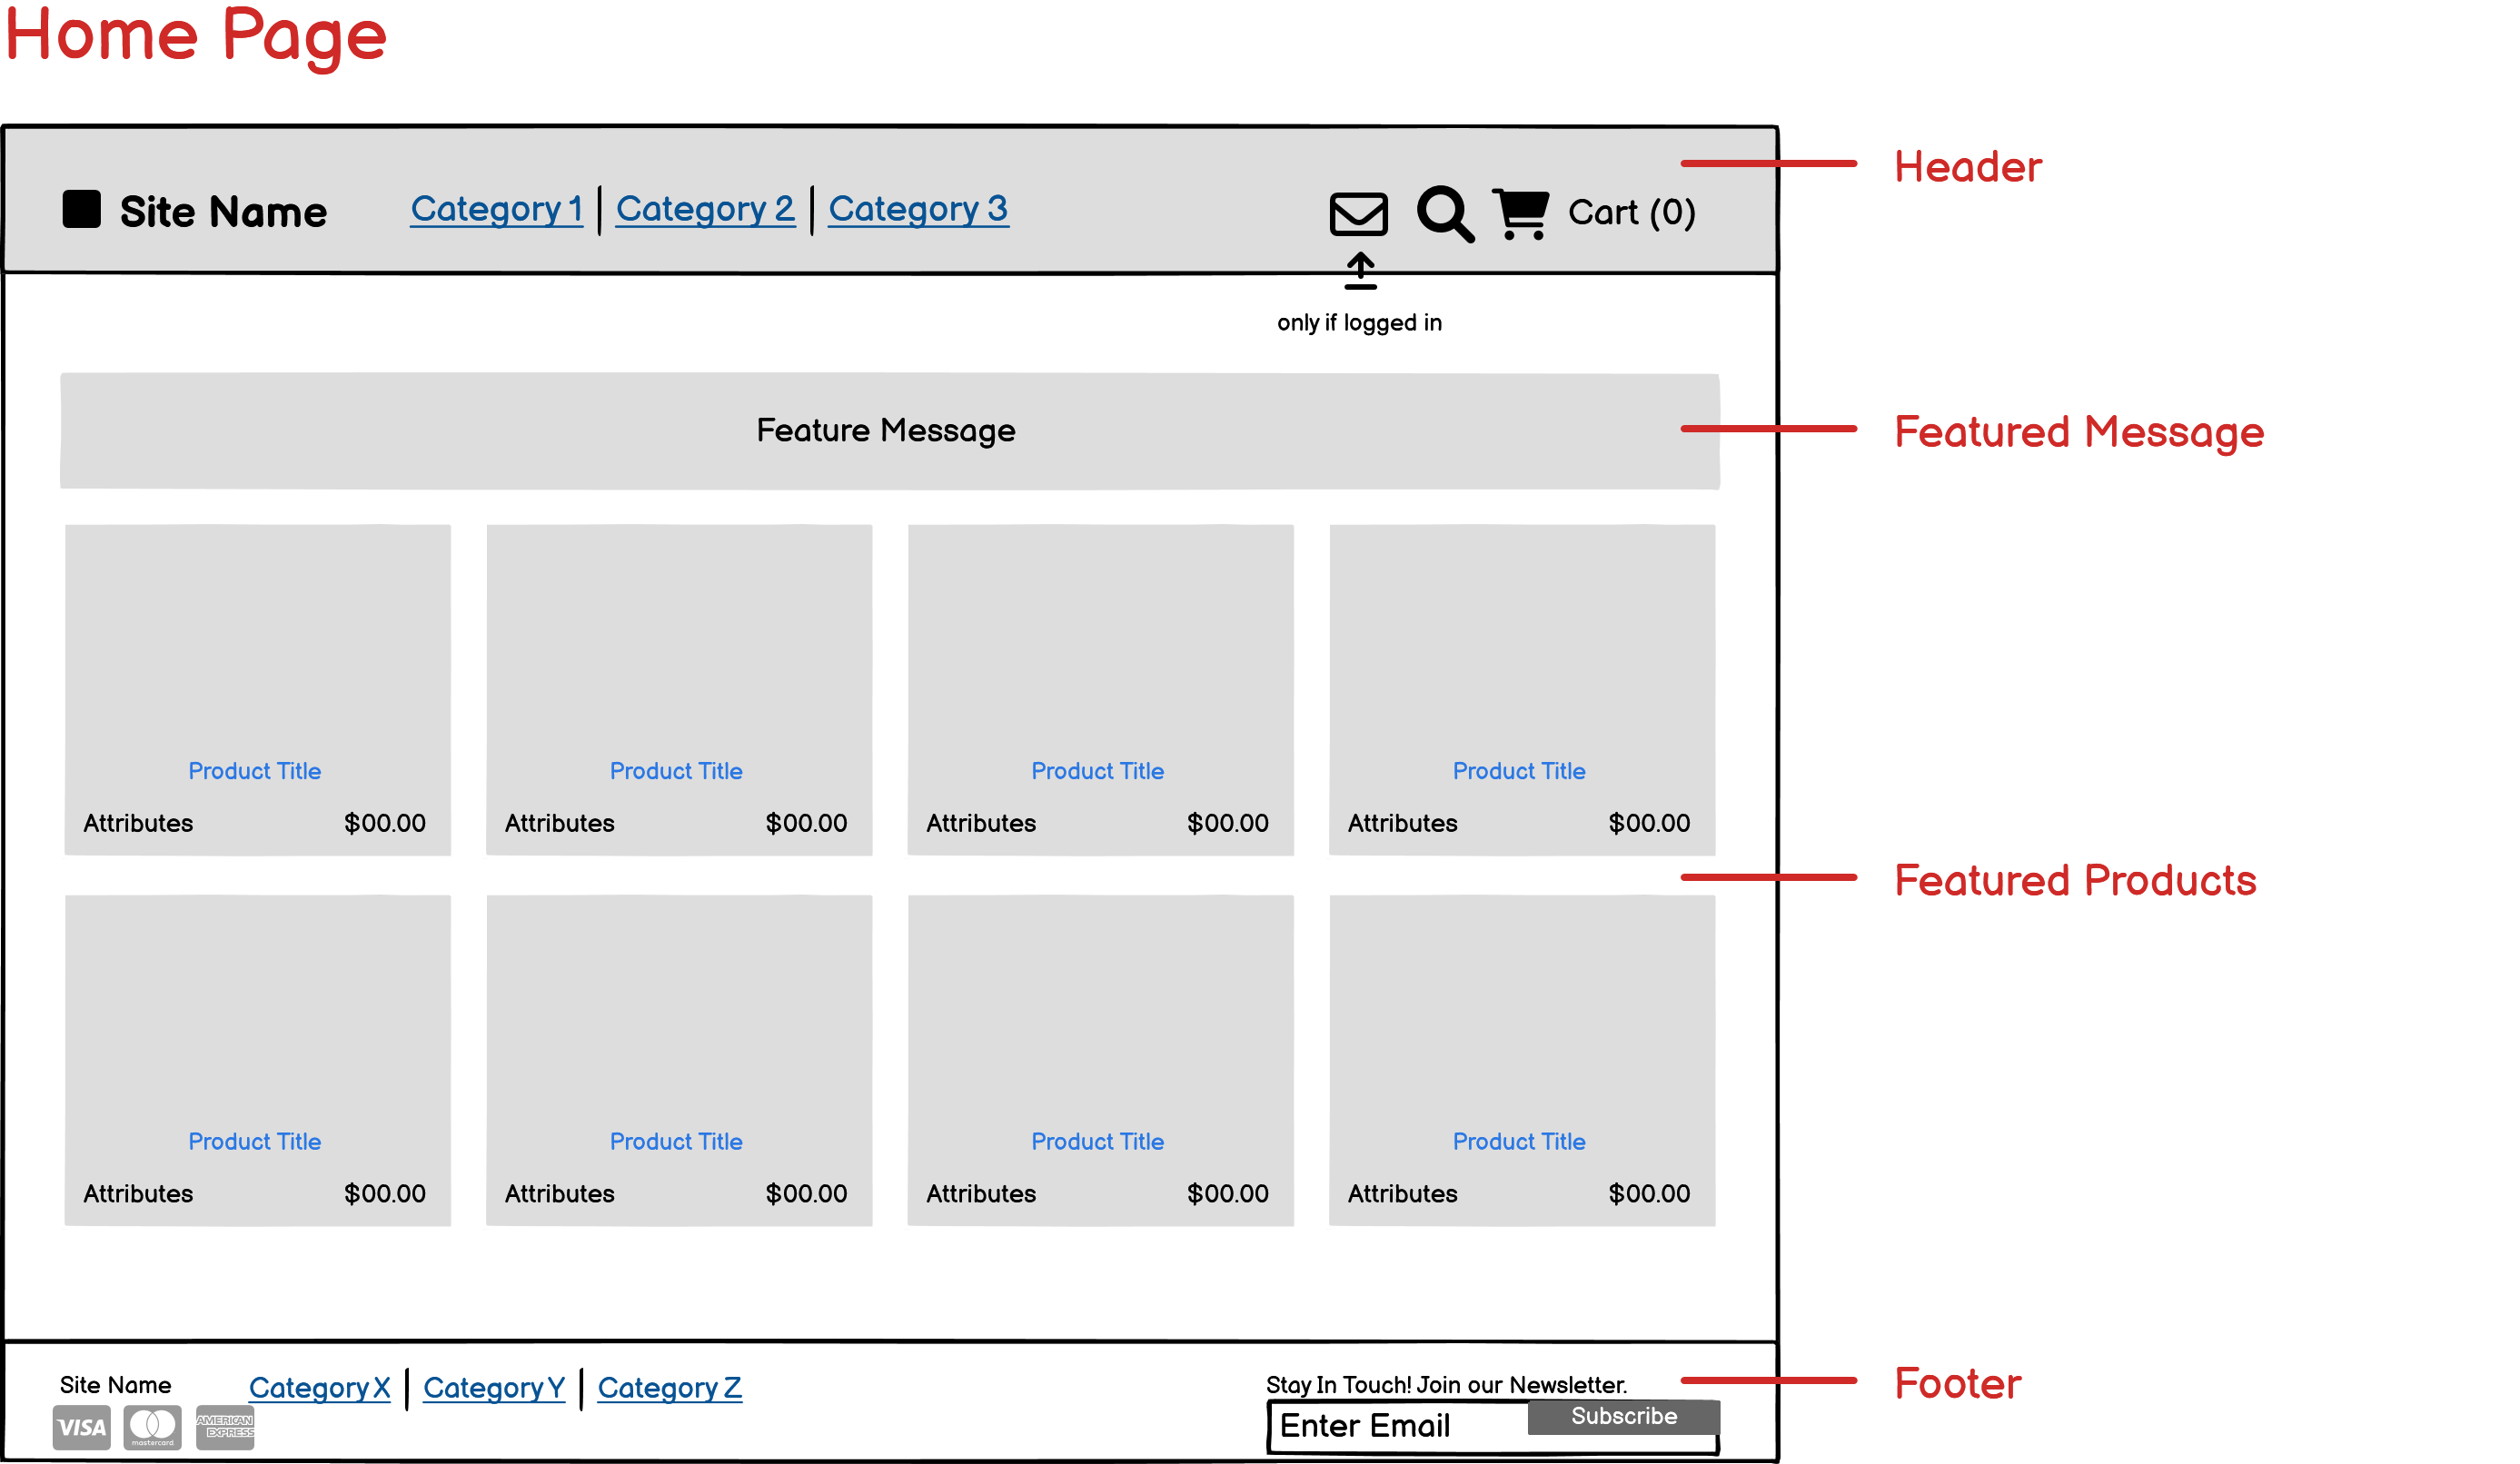
\includegraphics[scale=0.5]{logos/Images/pages/Home Page.png}

\begin{figure}[h]
    \centering
    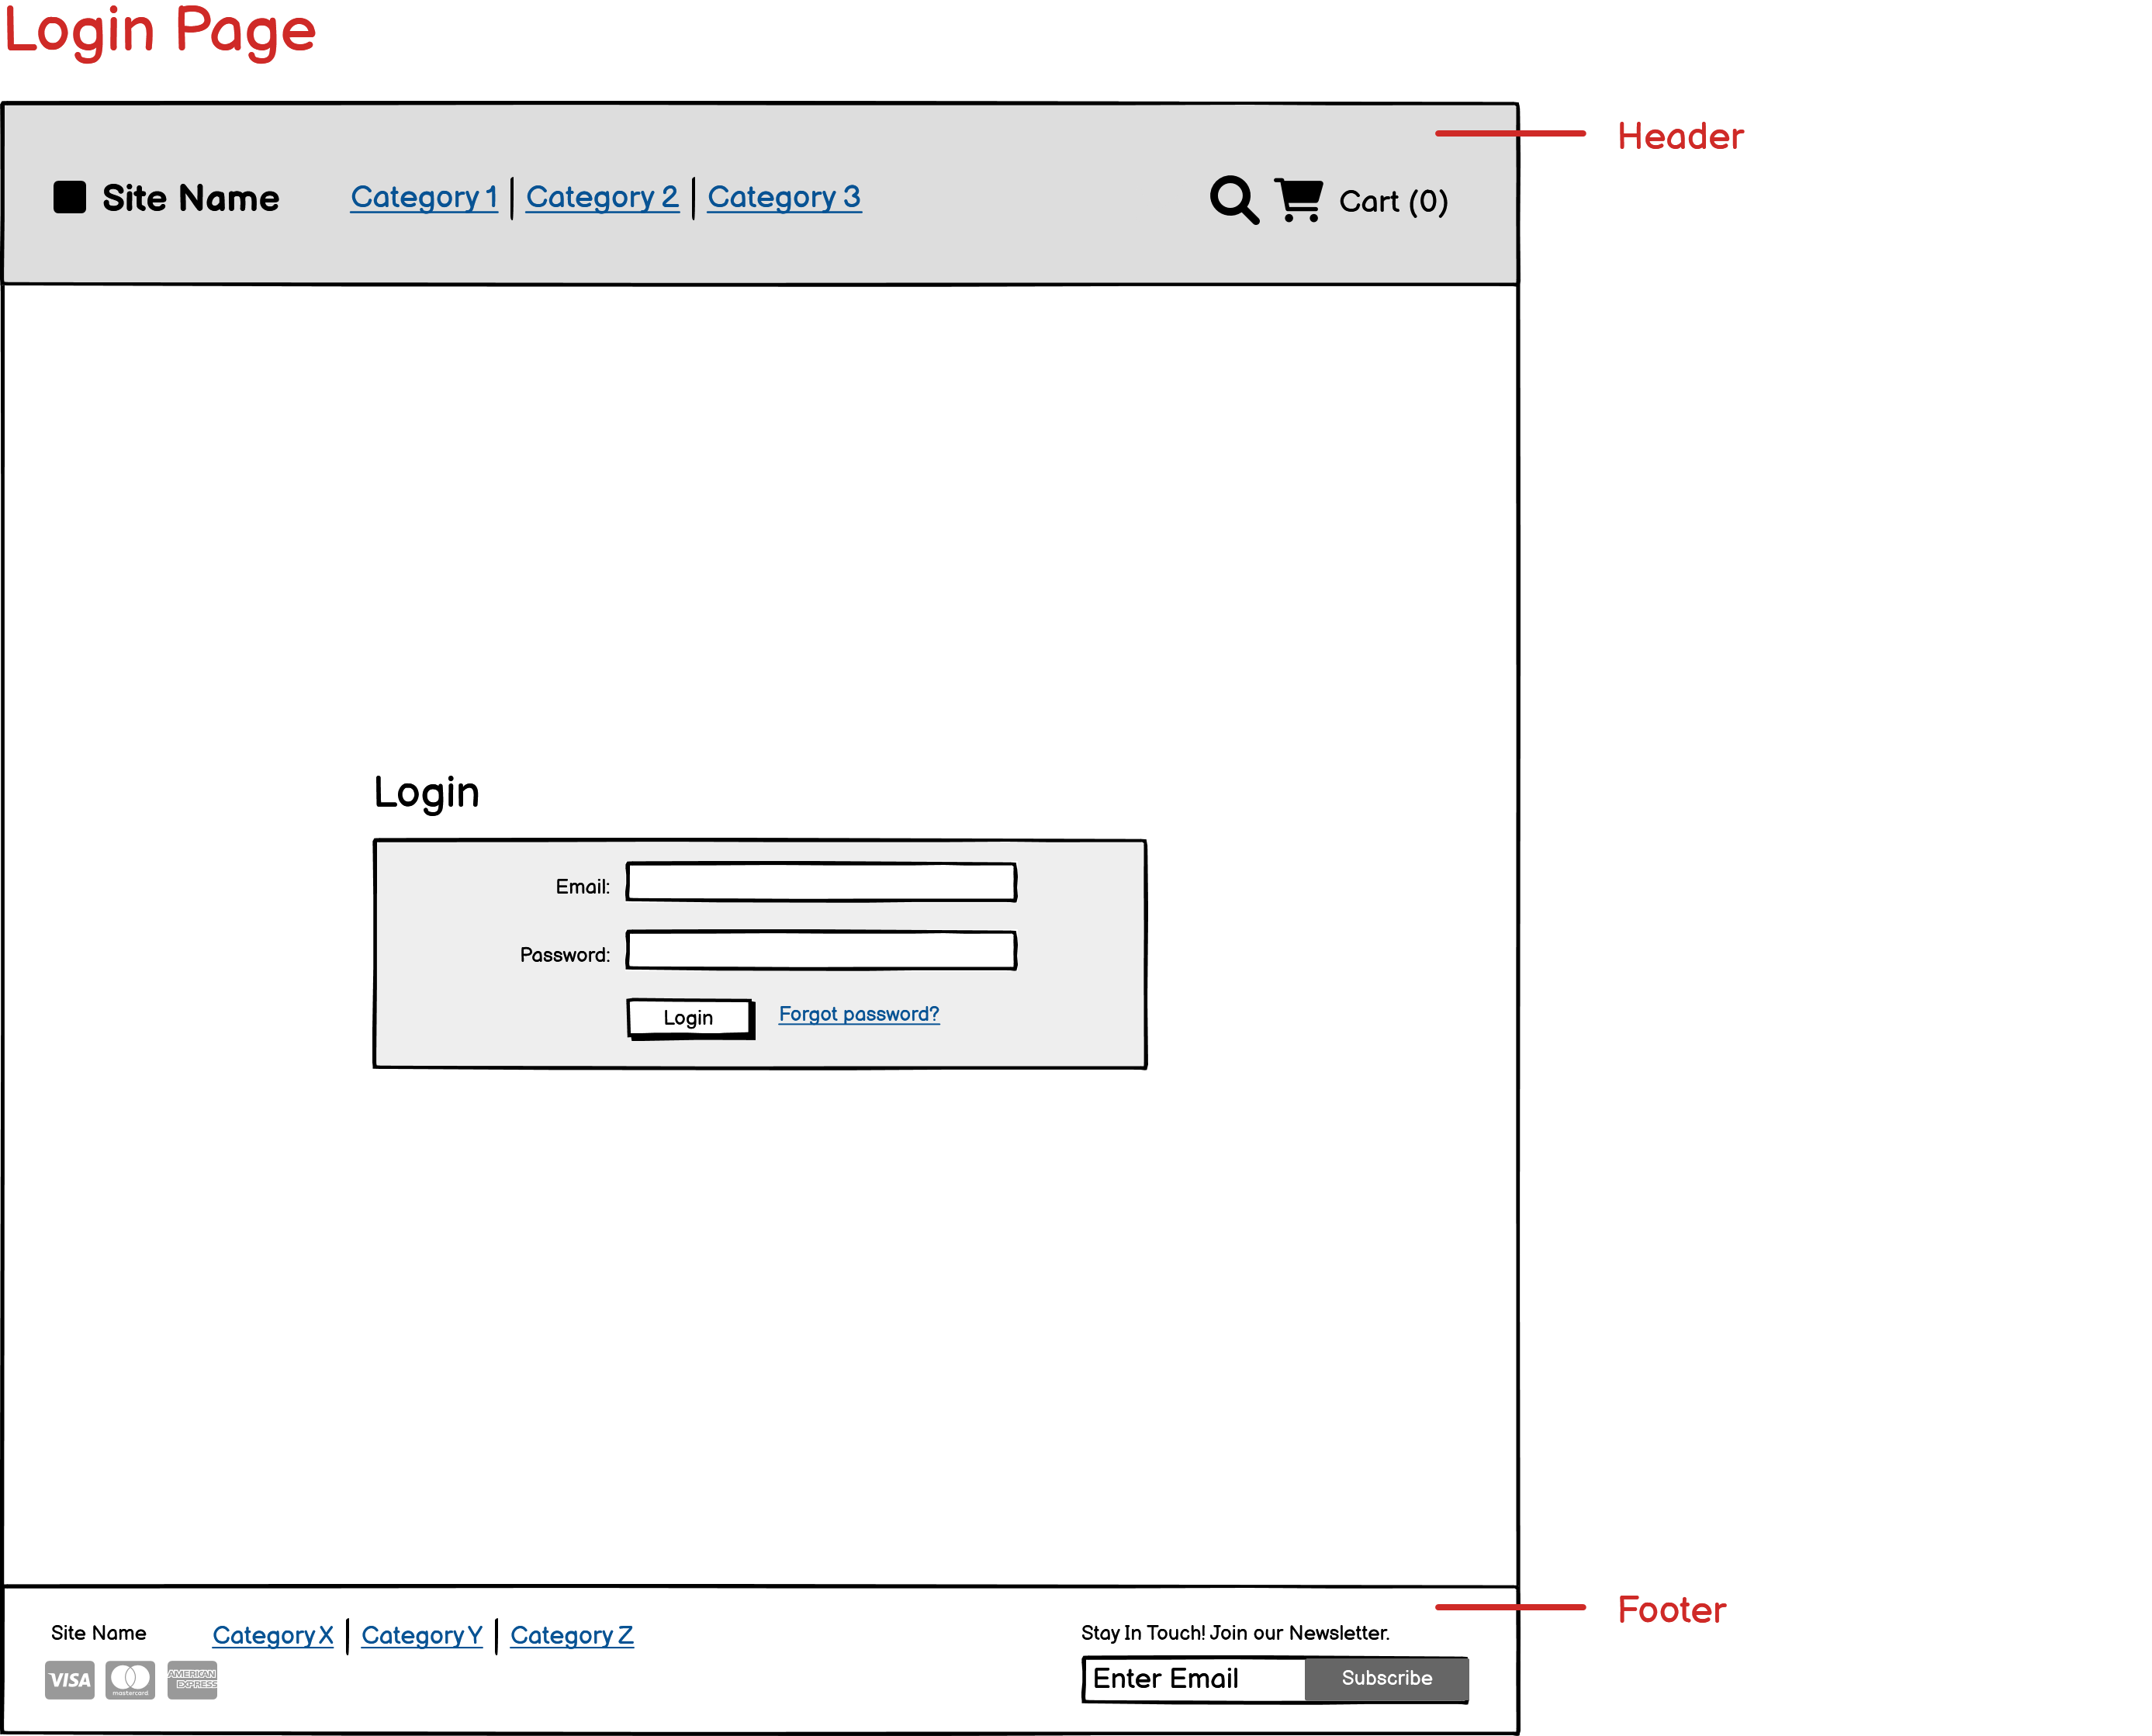
\includegraphics[scale=0.4]{logos/Images/pages/Login Page.png}
    \caption{Login Page}
    \label{fig:my_label}
\end{figure}
\hfill \break
This is a login page where users can log in to access their account. The login page contains two important fields: the email address and the password.\\\\
The email address is needed to ensure that the user is a registered user and to identify the account they are trying to access. The password is required to ensure that the user is the legitimate owner of the account and to protect the account from unauthorized access.\\\\
When a user attempts to log in to the login page, they must enter their email address and password in the appropriate fields. The website will then check if the email address and password are correct and if the account is active. If everything is correct, the user will be able to access their account successfully.